\documentclass{article}

% packages
\usepackage{blindtext}
\usepackage{titlesec}
\usepackage{booktabs}
\usepackage{graphicx}
\usepackage{xcolor}
\usepackage{indentfirst}
\usepackage{subcaption}

\usepackage{hyperref}
\hypersetup{
    colorlinks=true,
    linkcolor=blue,
    filecolor=magenta,
    urlcolor=cyan,
    pdftitle={DemoEqualityContribution},
    pdfpagemode=FullScreen,
}

% preference for indentation
\setlength\parindent{12pt}

% Title & Body begins
\begin{document}

\title{Demonstration Equality Contribution}
\author{Adam Wu, Nathaniel Laurente, Jackson Kennedy, Neena Ngyuen}
\maketitle

\section{Adam Wu}

\subsection{Github Setup and CI Checks}
I started working on setting up the Github and worked on building a CI checks, rulesets, and artifact for compiling our LaTeX file. This helps to ensure that the LaTeX file is always compiling during the development process. Furthermore, it prevents other members from pushing code that breaks the LaTeX file. 

\subsection{Design For Assembly}
On the design for assembly portion for submission 2, I worked on the CAD of the aesthetic prototype of the smart lock. I tried my best to make sure that the parts were designed in a way that they could be easily assembled and disassembled.

\begin{figure}[htbp]
    \centering
    \begin{subfigure}[b]{0.48\textwidth}
        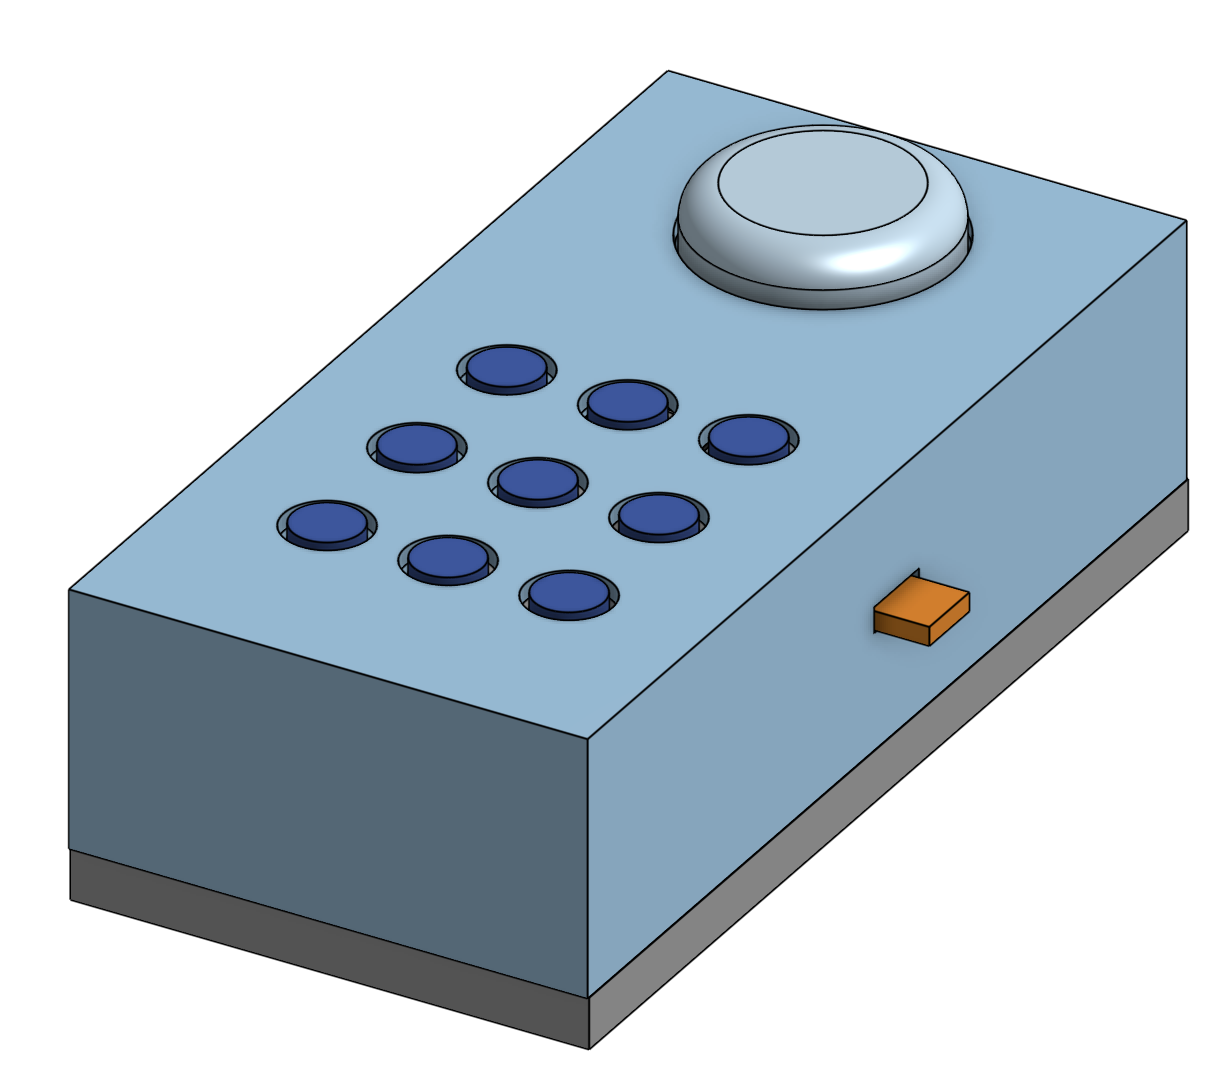
\includegraphics[width=\textwidth]{../submission3/img/isoView.png}
        \caption{Isometric View}
        \label{fig:isoView}
    \end{subfigure}
    \hfill
    \begin{subfigure}[b]{0.48\textwidth}
        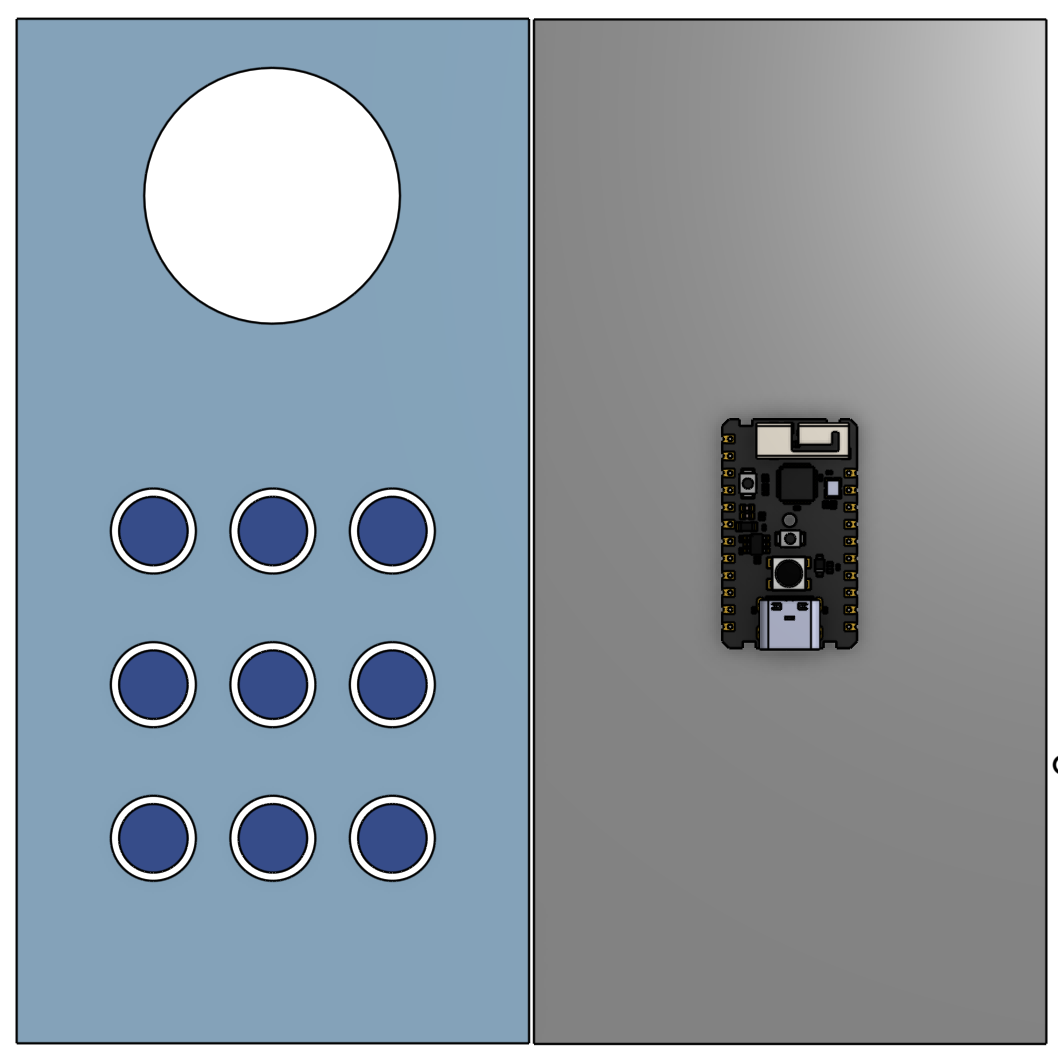
\includegraphics[width=\textwidth]{../submission3/img/topView.png}
        \caption{Top View}
        \label{fig:topView}
    \end{subfigure}
    \caption{First lock design}
\end{figure}

\subsection{Setting up ESP32-C3 toolchain (ESP-IDF)}
Since I am planning to work with the ESP32-C3, I started setting up the ESP-IDF toolchain on my local machine. I also started working on the initial setup of the ESP32-C3 to work with the "Hello World" example. Furthermore, I put in my researched information on the ESP-IDF documentation on where we can get started to connect to the WI-FI and to connect to Firebase.

\begin{enumerate}
    \item ESP-IDF have examples on basic wifi connection:
    \begin{itemize}
        \item in: \texttt{esp-idf/examples/wifi/getting\_started/station}
    \end{itemize}
    \item ESP-IDF also have examples on connecting to servers
    \begin{itemize}
        \item in: \texttt{esp-idf/examples/protocols}
    \end{itemize}
    \item We might also need to get another library for firebase connection
    \begin{itemize}
        \item link to firebaseClient: \url{https://github.com/mobizt/FirebaseClient}
        \item Another one: \url{https://github.com/dahmadjid/Firebase-idf}
    \end{itemize}
\end{enumerate}

\subsection{Gantt Chart}
For submission 2, I worked on the Gantt chart. I utilized a gantt chart template from a youtube video and modified it to fit our project. I also added the tasks that we need to complete for the next quarter.

\subsection{Test Plan}
I helped editing the test plans for ideas that was not put on the paper. I also helped with the formatting of the test plan.

% TODO: input what you have done on a separate file

\section{Jackson Kennedy}

\subsection{IOS App}
As a sector of the project, I took on the IOS portion of the project as my own task.
\\\\
Pictured below is the main screen where the user will lock/unlock the smartLock. The phone screen you see is not a simple concept drawing, but is actually coded. The buttons both work, and reflect the lock status in the database. Attached is a picture of the database reflecting the status, 1 - unlocked, 0 - locked. This is significant because now, data can be pulled from the cloud in real time.
\begin{figure}[h]
     \centering
     \begin{subfigure}{0.3\textwidth}
         \centering
         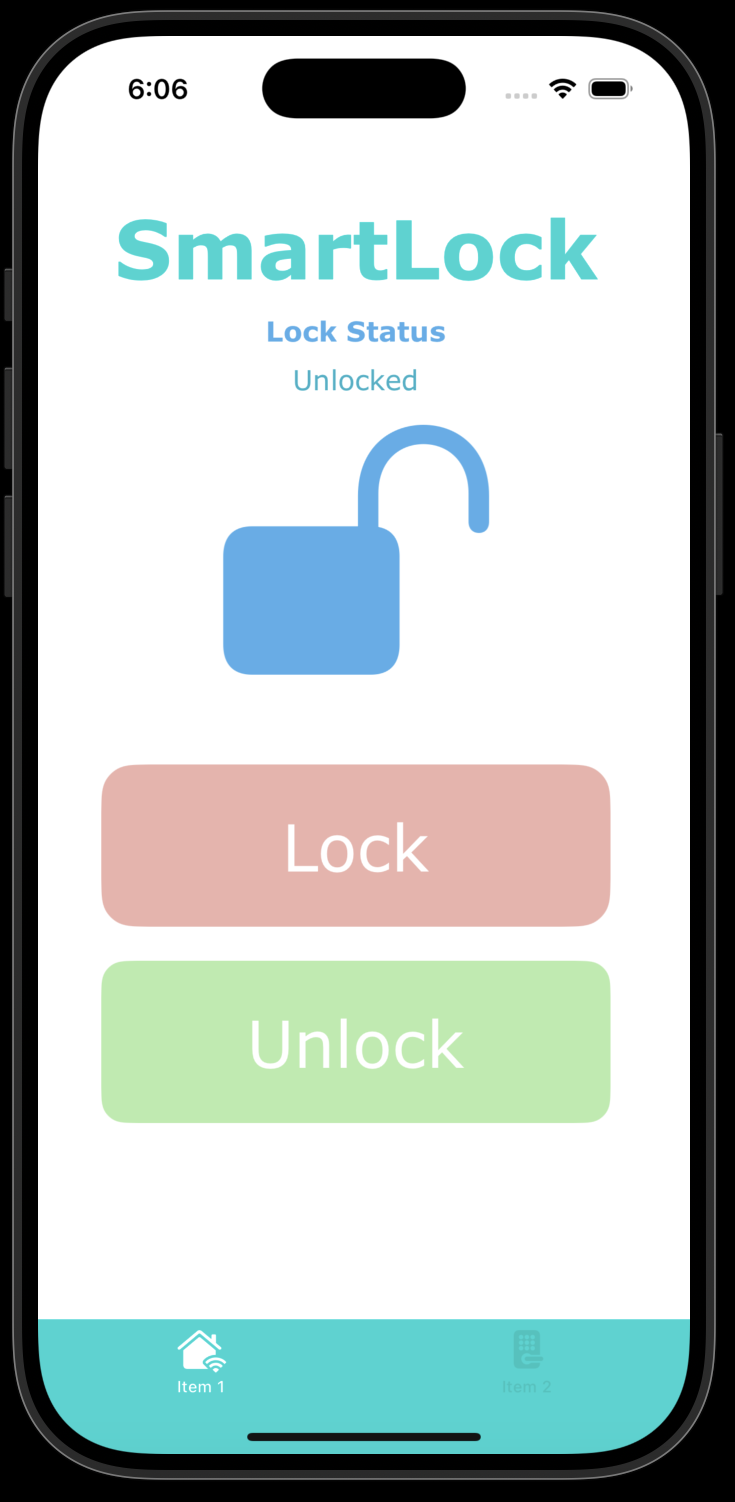
\includegraphics[width=\linewidth]{./img/unlockedPage.png}
         \caption{}
         \label{fig:1a}
     \end{subfigure}
     \begin{subfigure}{0.6\textwidth}
         \centering
         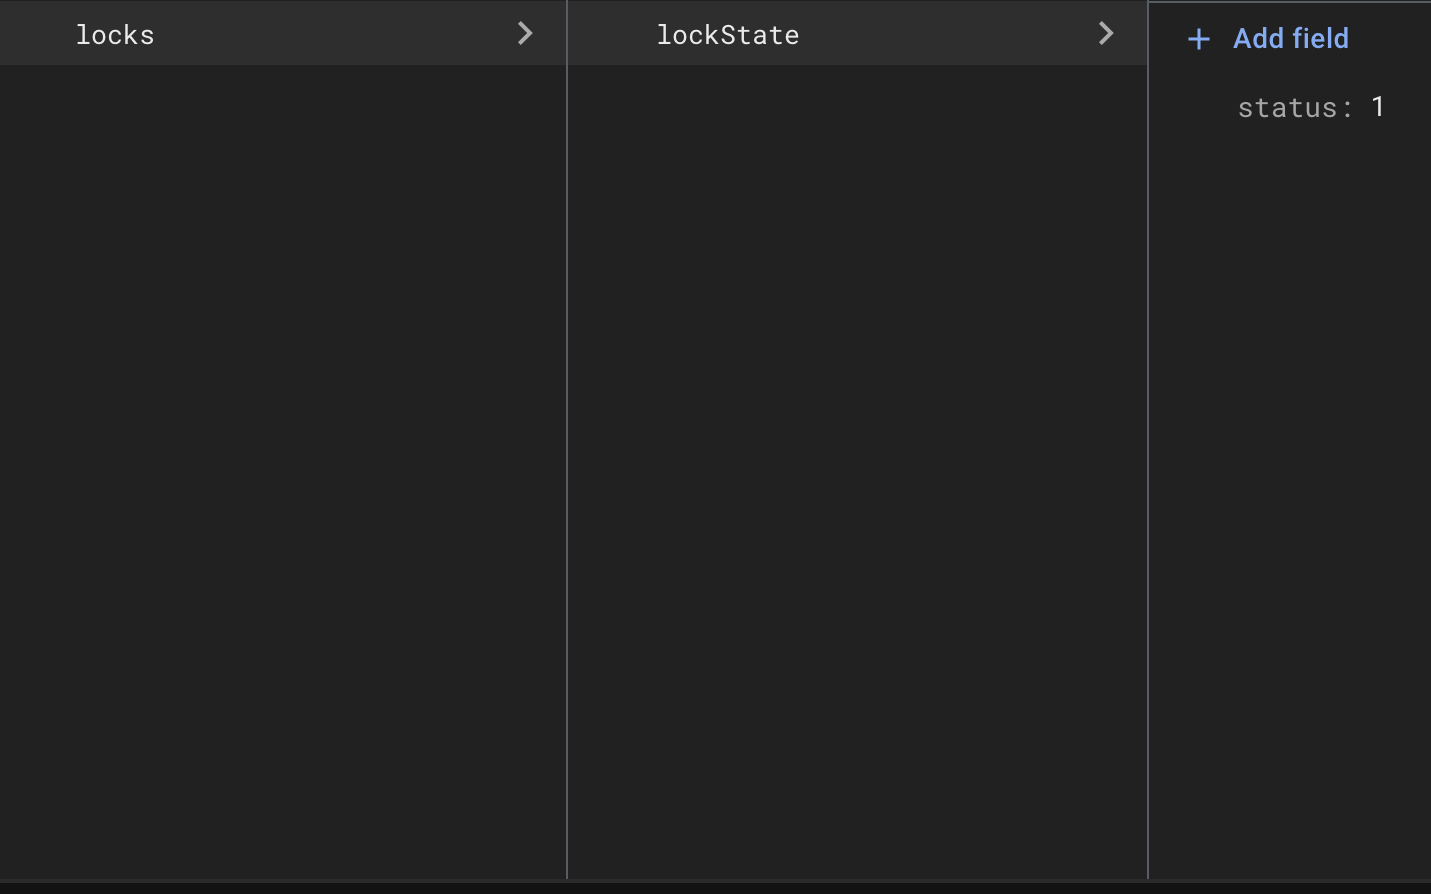
\includegraphics[width=\linewidth]{./img/lockState.png}
         \caption{}
         \label{fig:1b}
     \end{subfigure}
     \caption{Unlocked State on mobile device reflecting in cloud database.}
     \label{fig:1}
\end{figure}
\newpage
Additionally, I have set up the framework and programmed another screen that is accessible via the toolbar on the bottom of the screenshot. This is not yet connected to any database, but I populated it with a sample array of sample pins that I will later set up for secure user generation. This sets up the app for easy configuration down the line, where user generated pins can be used to populate the array and present as a part of a scrollable view on the app to consolidate the user's data.

\begin{figure}[htbp]
    \centering
    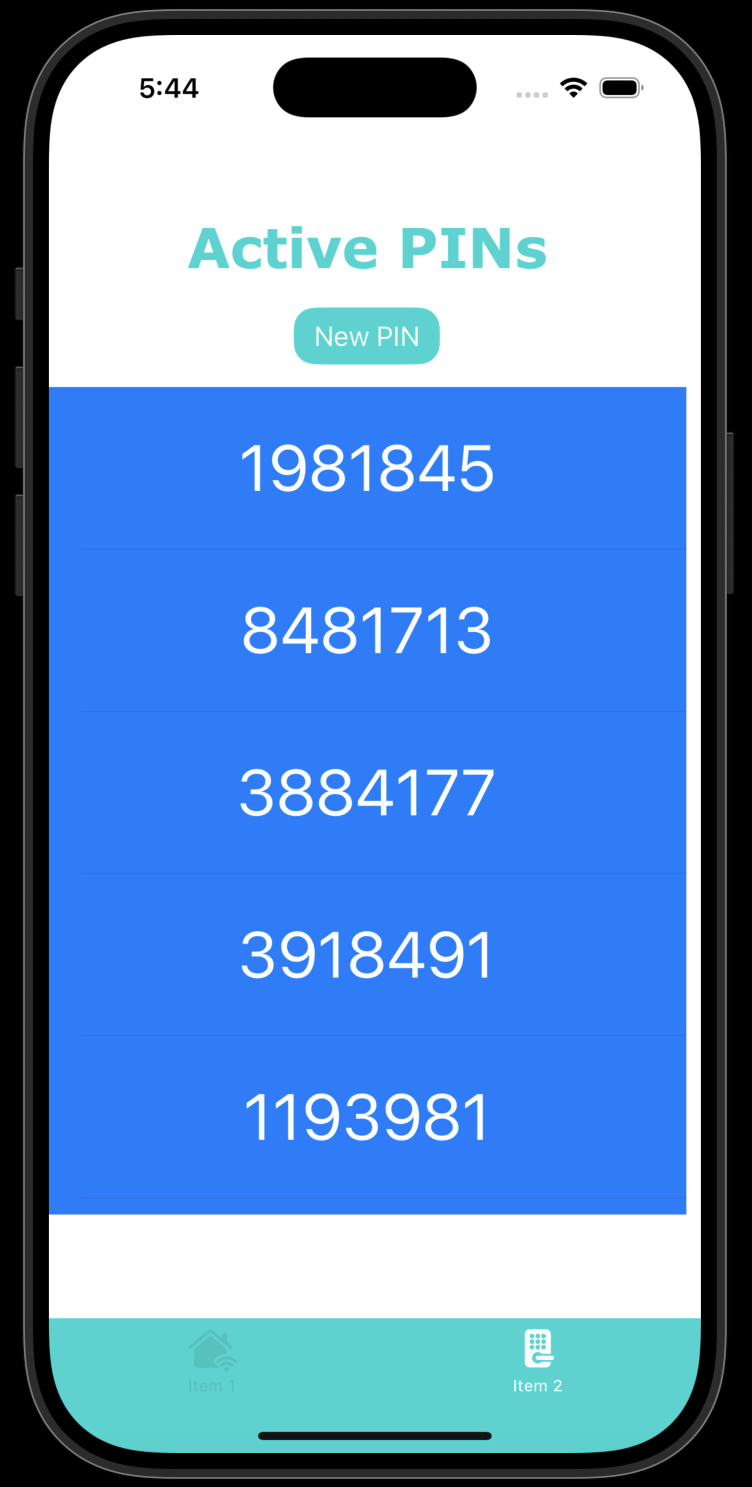
\includegraphics[width=0.185 \linewidth]{./img/pinPage.png}
    \caption{Pin Tab}
    \label{fig:pin}
\end{figure}
One of the main requirements for the end of this quarter was to get the phone communicating with the cloud, which I have been successful in transmitting data from the IOS device to the cloud provider and database.

\subsection{Test Plan}

On top of the mobile app, I helped to contribute to the test plan by writing a lot of the test plan based on project requirements. This includes things like hardware testing, and software communication testing.

\subsection{Morphological Chart}

I completed my section in the Morphological chart and added my design ideas and communication protocols.

\subsection{Mind Maps}

I helped to create the mind map by adding relevant sections and subsections with related technologies and ideas. This mind map helped us to push forward to strategize our different sections and account for different features and fields involved in the project.
% TODO: input what you have done on a separate file

\section{Neena Nguyen}

\subsection{Personas}
I designed a few user personas to represent the type of consumer likely to use or to benefit from the project prototype. 

% \subsection*{Submission 2}

\subsection{Ethics Statement}
I outlined the ethics statement for our smart lock, taking into consideration responsible design and implementation. I recognized potential risks with things like user privacy and data security to reassure users and recognize their concerns and needs for transparency.

\subsection{Lifecycle Assessment}
I designed a lifecycle assessment for the smart lock to evaluate its environmenmenal impact from sourcing materials to end of life disposal.

\subsection{Understanding ESP32 Integration with Firebase}
I read up on documentation for connecting the ESP32C3 to Wi-Fi and Firebase with the goal of exploring how our smart lock would utilize a cloud to authenticate users.

% TODO: input what you have done on a separate file

\section{Nathaniel Laurente}

\subsection{Goal Statement}
    I worked on coming up with a Goal Statement that fits the new project.

\subsection{ESP32-C3 Communication With OLED Display}


\begin{figure}[!ht]
    \centering
    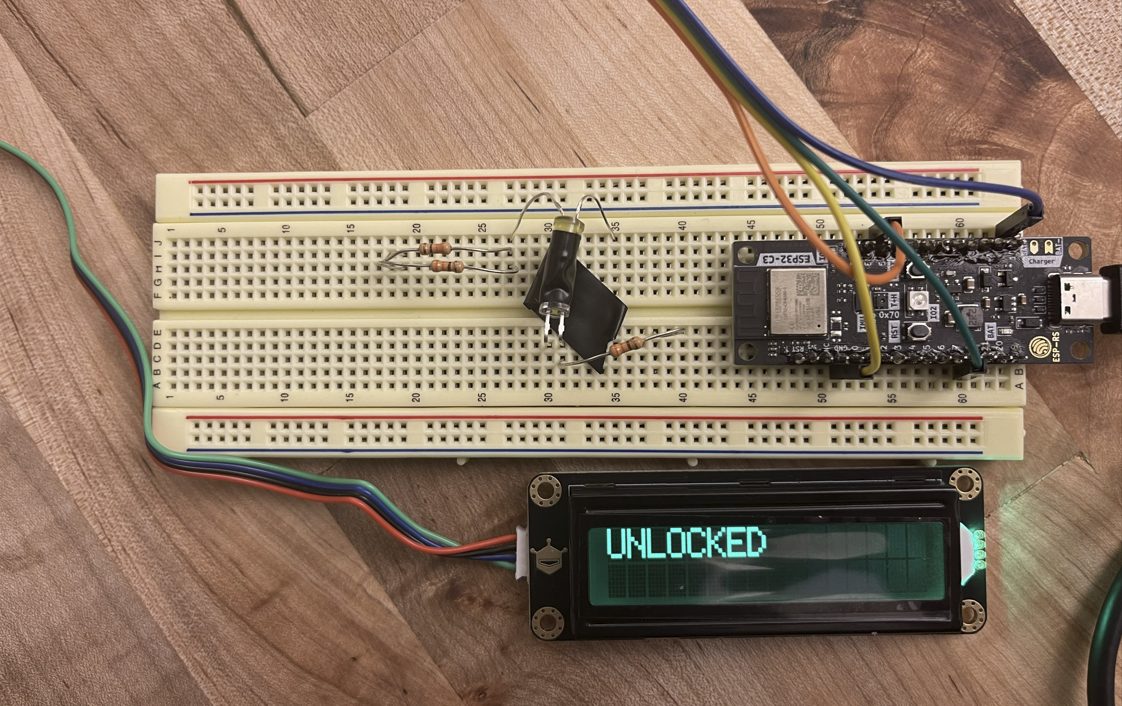
\includegraphics[width=140mm,scale=0.5]{./img/disp.png}
    \caption{ESP32-C3 Established Communication with OLED RGB Display}
    \label{fig:enter-label}
\end{figure}

    I was able to configure the ESP32-C3 to display "Unlocked" and "Locked." I set the toolchains such that there will be no issue sending signals from ESP32-C3 too the OLED dislay with minimal delay. My testing interface involved making sure there were no leaks and data was being power efficient when sending signals.

\subsection{Design For Manufacture}
    In the design for manufacture, I meticulously evaluated and selected components that strike an optimal balance between power efficiency and cost-effectiveness. This careful selection ensures that our auto-locking door system is not only marketable but also operates with minimal power consumption, thereby enhancing its overall functionality and sustainability.

\subsection{Decision Tables}
    I made the decision tables for the weights of the necessary parameters for our auto-locking door. This allowed our team to decide on a final design out of the three options we had come up with for our design. For an auto-locking door design, of course security was the number 1 concern for our project, and we decided to go for an option that prioritized security while maintaining cost efficiency.


\section{Work Contribution as a Group}

\subsection*{Need \& Goal Statements}
Our team collaboratively decided on the need and goal statements for our smart lock project. We identified the situations in which our smart lock would be most relevant, defined the problem, identified who our main consumers would be and their requirements, and established a reachable goal to help us meet those user requirements.

\subsection*{6-3-5}
We all contributed to the brainstorming process using the 6-3-5 method, rotating between 4 rounds until each of us had added on to everyone else's initial thought. 

\subsection*{Brainstorming}
We all contributed to the overall brainstorming for our smart lock by writing on the same document any ideas we had for our respective smart locks. We generated any and all possibilities, including design features we'd seen previously. 

\subsection*{Morphological Charts}
We each drew up our own visions for the smart lock and key to get a better sense of how our ideas aligned and differed.

\subsection*{Mind Maps}
We created and organized a mind map for our smart lock. We visually structured our ideas to help each other see connections between different features so our approach could be more well-rounded.

    % \subparagraph{Goal Statement}
    % Nathaniel worked on this part of the submission.





% During week 7, our team worked mainly on new design objectives and the need statement due to the unexpected leave of one of our teammates. Due to this unexpected leave of absence, our team was compelled to switch projects halfway through the quarter. We came up with a new project to work on for the next two quarters and had to redesign our project proposal. We also had to reassign roles and responsibilities to accommodate the new project. Below in this section, we will provide descriptions on what we all worked on during week seven.

% Below is our submission 1 before the switch to our new project idea. In submission 1, we designed the personas, need statement, goal statement, and Design Objectives in relation to the lithography machine idea we had for the first half of the quarter.

% % Submission 1 contribution details
% \subsection{Submission 1 Contribution}

% \subparagraph{Personas} 
% Neena worked on this part of the submission.

% \subparagraph{Need Statement}
% We all thought about the need statement and came up with a general idea of what we wanted to do. We all contributed to the need statement.

% \subparagraph{Goal Statement}
% Nathaniel worked on this part of the submission.

% \subparagraph{Design Objectives In Words}
% Jackson worked on this part of the submission.

% \subparagraph{Design Objectives As Quantified Table}
% Adam worked on this part of the submission.


% % "Work" that we were doing for the actual project
% \subsection{Brainstorming New Project Ideas}



% \section{Nathaniel Laurente}

% % Submission 2 contribution details
% \subsection{Submission 2 Contribution}
% \begin{itemize}
%     \item \textbf{Brainstorming}
%     \begin{itemize}
%         \item Adam Wu, Nathaniel Laurente, Jackson Kennedy, Neena Ngyuen
%     \end{itemize}
    
%     \item \textbf{6-3-5 method}
%     \begin{itemize}
%         \item Adam Wu, Nathaniel Laurente, Jackson Kennedy, Neena Ngyuen
%     \end{itemize}
    
%     \item \textbf{Morphological Charts}
%     \begin{itemize}
%         \item Adam Wu, Nathaniel Laurente, Jackson Kennedy, Neena Ngyuen
%     \end{itemize}
    
%     \item \textbf{Mind Maps}
%     \begin{itemize}
%         \item Adam Wu, Nathaniel Laurente, Jackson Kennedy, Neena Ngyuen
%     \end{itemize}
        
%     \item \textbf{Design Objectives As Quantified Table}
%     \begin{itemize}
%         \item Adam Wu
%     \end{itemize}
% \end{itemize}
% % end contribution from submission 1   


% \section{Week 9}



\end{document}
